\documentclass[conference]{IEEEtran}
% \IEEEoverridecommandlockouts
% The preceding line is only needed to identify funding in the first footnote. If that is unneeded, please comment it out.
\usepackage{cite}
\usepackage{amsmath,amssymb,amsfonts}
\usepackage{algorithmic}
\usepackage{graphicx}
\usepackage[brazilian]{babel}
\usepackage[utf8]{inputenc}
\usepackage{textcomp}
\usepackage{xcolor}
\def\BibTeX{{\rm B\kern-.05em{\sc i\kern-.025em b}\kern-.08em
    T\kern-.1667em\lower.7ex\hbox{E}\kern-.125emX}}
\begin{document}

\title{Reconhecimento de Gestos\\
%{\footnotesize \textsuperscript{*}Note: Sub-titles are not captured in Xplore and
%should not be used}
%\thanks{Identify applicable funding agency here. If none, delete this.}
}

\author{\IEEEauthorblockN{1\textsuperscript{st} Raphael Ramos}
\IEEEauthorblockA{\textit{Ciência da Computação} \\
\textit{Universidade de Brasília}\\
Brasília, Brasil \\
raphael.soares.1996@gmail.com}
\and
\IEEEauthorblockN{2\textsuperscript{nd} André Luis Souto}
\IEEEauthorblockA{\textit{Engenharia de Computação} \\
\textit{Universidade de Brasília}\\
Brasília, Brasil \\
andresouto.as@gmail.com}
\and
\IEEEauthorblockN{3\textsuperscript{th} Rafaela Sinhoroto}
\IEEEauthorblockA{\textit{Engenharia Mecatrônica} \\
\textit{Universidade de Brasília}\\
Brasília, Brasil \\
rsinhoroto@hotmail.com}
}

\maketitle

\begin{abstract}
Gestos são parte da comunicação não verbal diária, dessa forma, provendo um jeito inovador e natural de interação com o computador. Logo, reconhecimento de gestos tem aplicações largas na área de computação, como interação humano-computador, linguagem de sinais e jogos. Neste trabalho, duas abordagens de reconhecimentos de gestos, uma baseada em redes neurais convolucionais e outra baseada em parâmetros do formato da mão, são testadas com o \textit{Marcel dataset} e têm sua acurácia comparadas.   
\end{abstract}

\begin{IEEEkeywords}
Processamento de Imagem, Redes Neurais Convolucionais, Reconhecimento de Gestos, Parâmetros de Forma.
\end{IEEEkeywords}

\section{Introdução} 
Neste trabalho foram comparados dois modelos diferentes para realizar reconhecimento de gestos: redes neurais convolucionais (CNN) e reconhecimento baseado em parâmetros de forma \cite{shapeparameters}.
Para fazer o treinamento e o teste dos nossos modelos, nós usamos o \textit{Marcel dataset}~\cite{dataset} que consiste de 6 sinais de mão (A, B, C, FIVE, POINT, V) executados por 24 pessoas em três tipos diferentes de \textit{backgrounds}. Pessoas e \textit{backgrounds} diferentes foram usados para aumentar a diversidade e a informação contida no \textit{dataset}. Em termos de \textit{background}, as imagens no \textit{Marcel dataset} foram capturadas em um \textit{background} uniforme com luz, um uniforme escuro e um \textit{background} complexo variado. Devido ao número diferente de pessoas incluídas na criação desse dataset há também variação no formato e tamanho da mão, além de rotações e mudanças na forma que os sinais são executados. Este dataset contém 4872 imagens de treino e 658 de teste.

\par Por fim, a acurácia dos dois métodos utilizados é comparada a fim de determinar o mais eficiente para o dataset utilizado, considerando fundo da imagem e gestos reconhecidos. 


\section{Trabalhos Relacionados}
Redes neurais profundas são a base dos resultados do estado da arte para reconhecimento de imagens~\cite{simonyan}, detecção de objetos~\cite{girshick2014rich}, reconstrução tridimensional de objetos~\cite{choy20163d}, reconhecimento de faces~\cite{deepface}, reconhecimento de discurso~\cite{graves}, \textit{machine translation}~\cite{sequence}, geração de legendas de imagens~\cite{vinyals2015show}, tecnologia de carros autônomos~\cite{huval2015empirical}, entre outros. Entretanto, treinar uma rede neural profunda é uma problema de otimização global difícil. Por isso, para o presente trabalho foi utilizado o método de \textit{machine learning} conhecido como \textit{transfer learning}~\cite{Pan2010ASO}. \textit{Transfer learning} é um metodo onde um modelo desenvolvido para uma tarefa é reusado como ponto de partida para um modelo em outra tarefa. Esse método foi utilizado neste projeto para a inicialização dos pesos visto que ele permite progresso rápido e performance melhorada para modelar a tarefa requerida.
\par O outro método utilizado para comparação, reconhecimento baseado em parâmetros de forma, utiliza como referência o trabalho \cite{shapeparameters} com algumas correções e adaptções para o \textit{dataset} utilizado. Para reconhecimento de gestos, são utilizados apenas parâmetros baseados no formato da mão, como centro de massa, orientação, e posicionamento dos dedos. Logo, cor da pele e textura não são considerados. No trabalho anterior, são analisadas apenas gestos em fundo branco e sem a presença de partes da roupa cobrindo o pulso, o que facilita o processo de segmentação da mão e detecção da orientação do gesto. Nesta abordagem, foram feitas alterações para permitir a segmentação da mão em fundos variados, e com o pulso coberto.


\section{Soluções Propostas}

\subsection{Redes Neurais Convolucionais}
Temos como vantagem do uso de aprendizado profundo a desnecessidade de engenharia de características -- a própria rede o faz. Como contrapartida, necessita-se de uma grande quantidade de exemplos de treinamento. Neste trabalho isso foi mitigado pelo uso de \textit{data augmentation}, e transferência de aprendizado ao usar pesos pré-treinados para uma maior e mais desafiadora tarefa de classificação de imagens em 1000 classes: a
ImageNet \cite{imagenet_cvpr}. Foram avaliados dois modelos de redes neurais neste trabalho: \textit{Xception}~\cite{xception} e \textit{Inception ResNet V2}~\cite{szegedy2017inception}.

A \textit{Inception ResNet V2}~\cite{szegedy2017inception} é uma rede neural convolucional que faz convoluções fatorizadas e regularizações. Devido a imensa variação na localização da informação em uma imagem, escolher o tamanho do kernel ideal para realizar operações de convolução, que destacam partes salientes da imagem, é uma tarefa difícil. Um tamanho de kernel maior é preferível para a informação que é distribuída mais globalmente, enquanto um kernel de tamanho menor é preferível para informação que é distribuída mais localmente. Para resolver esse problema, as redes da linha \textit{Inception} introduziram os módulos \textit{Inception}, que realizam convoluções em uma entrada com vários tamanhos de filtros além de realizar \textit{max pooling} para obter \textit{features} contidas em subregiões da entrada. Para a versão residual das redes \textit{Inception} (\textit{Inception ResNet V2}) foi utilizado blocos \textit{Inception} mais baratos que o modelo original

Na \textit{Xception} houve uma modificação na camada \textit{Depthwise Separable Convolution}. Nesta camada existe uma \textit{pointwise convolution} seguida por uma \textit{depthwise convolution} (ordem contrária no modelo \textit{InceptionV3}~\cite{inception}). \textit{Depthwise convolution} é a convolução espacial canal a canal. A convolução separável em profundidade (\textit{Depthwise convolution}) baseia-se em fatorizar a operação de convolução em duas camadas: uma convolução em profundidade que aplica um filtro para cada canal da entrada; e uma convolução por pontos (pointwise), de tamanho 1x1, responsável por criar novas características por combinações lineares dos canais de entrada e alteram a dimensão. Como resultado, são mais baratas computacionalmente sem perdas de performance significativas em relação às convoluções completas.
\subsection{Reconhecimento Baseado em Parâmetros de Forma} 
O algoritmo de reconhecimento baseado em parâmetros de forma segue os seguintes passos:
\begin{enumerate}
\item Segmentação da figura da mão utilizando \textit{k-means clustering};
\item Detecção de orientação da mão como horizontal ou vertical;
\item Extração de features relevantes para a classificação (centroide da mão, detecção do polegar, etc.);
\item Classificação a partir das informações obtidas nas etapas 1 a 3.
\end{enumerate}
\subsubsection{Segmentação}
A segmentação da mão é realizada utilizando \textit{k-means clustering} para agrupar os pixeis da mão em clusters separados dos pixeis do plano de fundo utilizando a distância euclidiana entre as diferentes cores de cada agrupamento. 
\par Para que o agrupamento funcione, primeiro é necessário transformar a informação de cor das imagens do espaço RGB para o espaço de cor L*a*b*, um espaço de cor baseado em um canal de luminosidade e dois canais cromáticos que permite que a diferença entre duas cores seja dada pela distância euclidiana entre elas. Os dois canais de cor, a* e b*, são baseados na teoria de cores opostas, onde duas cores não podem ser verdes e vermelhas ao mesmo tempo, nem amarelas e azuis ao mesmo tempo. 
\par Após essa transformação, é necessário estabelecer a quantidade de centroides para o \textit{k-means} classificar. Em imagens com condições uniformes (contendo apenas a mão realizando o gesto e um fundo plano, sem detalhes e de cor distinta a de pele), 2 centroides são suficientes para uma boa segmentação. Porém, em casos gerais, mais complexos, são utilizados 5 centroides para que o agrupamento não junte pedaços da mão com informação irrelevante de fundo. 
\par A técnica do \textit{k-means} funcina melhor com imagens maiores em que há maior distinção dos pixeis da mão para os de fundo. 
\subsubsection{Orientação}
\par Uma vez segmentada a mão, é necessário determinar sua orientação, vertical ou horizontal. A detecção correta é importante pois a orientação influencia diretamente no método de identificação dos dedos.
\par Dada a mão segmentada de largura L e comprimento C, calcula-se a razão R entre tais medidas:

\begin{equation}\label{eqeq}
    R = \frac{C}{L}
\end{equation}

assim, tem-se as condições

\begin{equation}\label{eqeq}
    Orientação =
    \begin{cases}
      Vertical, & R > 1 \\
      Horizontal, & \text{Caso contrário}
    \end{cases}
\end{equation}

Portanto, caso o comprimento da mão segmentada seja maior que sua largura, a mesma encontra-se na vertical. E caso a largura seja maior que o comprimento, a orientação é horizontal.

\begin{figure}
\centering
  \centering
  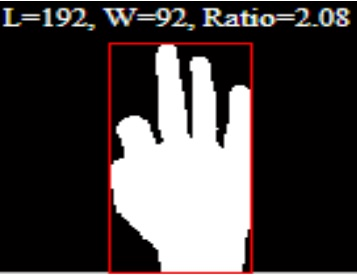
\includegraphics[width=.6\linewidth]{figs/vertical.jpg}
  \caption{Orientação vertical.}
  \label{fig:sub1}
  \centering
  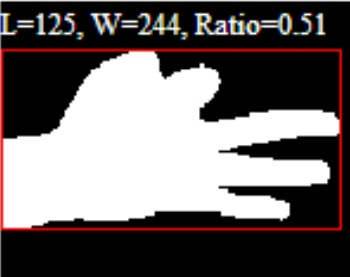
\includegraphics[width=.6\linewidth]{figs/horizontal.jpg}
  \caption{Orientação horizontal.}
  \label{fig:sub2}
\label{fig:test}
\end{figure}

\subsubsection{Extração de features}
\par Nesta etapa, são extraídas informações a respeito do centro de massa da mão (centroide), da presença ou não do polegar e do estado dos dedos, se estão levantados ou abaixados. Tais informações são usadas juntas na classificação e interpretação dos gestos.
\paragraph{Centro de Massa}
\par O centro de massa divide a imagem da mão em duas partes, uma parte contendo os dedos e outra não contendo. Tal divisão é feita no centro geométrico da imagem.
\par Para calcular o centroide, foi utilizado o momento da imagem, dado por 

\begin{equation}\label{eqeq}
    M_{ij} = \sum{\sum{x^{i}y^{j}I(x,y)}}
\end{equation}

onde $M_{ij}$ é o momento da imagem e I(x,y) é a intensidade na coordenada (x,y). Em resumo, o momento da imagem é a média ponderada das intensidades dos \textit{pixels} da imagem. Dado $M_{ij}$, foi possível calcular o centro de massa:
\begin{equation}\label{eqeq}
    {X_{c},Y_{c}= {\frac{M_{10}}{M_{00}},\frac{M_{01}}{M_{00}}}}
\end{equation}

onde $X_{c}$, $Y_{c}$ são as coordenadas do centroide e $M_{00}$ é a área da imagem binária.
\paragraph{Detecção de polegar}
\par Nesta etapa, há a identificação da presença ou não do polegar no gesto da imagem. Dados os limiares das laterais, obtidos na segmentação da mão, pega-se 30 \textit{pixels} para dentro da imagem partindo-se de cada uma das duas bordas laterais. Forma-se então dois retângulos de área 30 \textit{pixels} x comprimento da mão.
\par Calcula-se então a porcentagem de \textit{pixels} brancos dentro de cada retângulo em comparação com o total da imagem. Caso a porcentagem seja menor que 7\% em um dos lados, o polegar está presente neste lado. Caso nos dois retângulos conste uma porcentagem maior que 7\%, não há polegar no gesto. E caso nos dois lados haja menos de 7\% de \textit{pixels} brancos, também não há polegar no gesto.

\begin{figure}
\centering
  \centering
  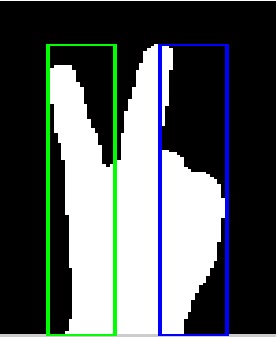
\includegraphics[width=.4\linewidth]{figs/thumb.jpg}
  \caption{Retângulos formados para detecção de polegar.}
\end{figure}


\paragraph{Identificação dos dedos}
\par Para a identificação do restante dos dedos são usados dois métodos. Primeiramente, percorre-se todo o contorno da mão segmentada a fim de marcar regiões de picos, pois tais regiões representam os dedos na imagem.
\par Com os picos detectados, no segundo método, calcula-se a distância euclidiana de todos os picos encontrados com o centro de massa. Dessa forma, tem-se todos os dedos identificados, porém, como alguns podem estar dobrados, todos os picos que tiverem distância euclidiana de valor menor que 75\% do maior valor, são declarados insignificantes, ou seja, dobrados.

\subsubsection{Classificação}
\par Por fim, dadas as informações obtidas na etapa de extração de features, gera-se um vetor de cinco bits onde cada bit representa o estado de cada dedo. Ou seja, caso ele se encontre no gesto, o bit correspondente é setado como 1. Caso contrário, é setado como 0. Na figura \ref{bits}, um exemplo de gesto com os cinco dedos levantados e abaixo o vetor de bits correspondente.

\begin{figure}
\centering
  \centering
  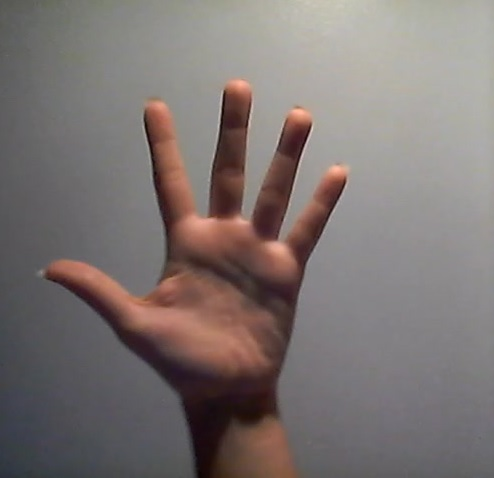
\includegraphics[width=.4\linewidth]{figs/bits.jpg}
  \caption{Gesto correspondente ao vetor de bits [1 1 1 1 1].}
\label{bits}
\end{figure}

\section{Resultados Experimentais}
\subsection{Redes Neurais Convolucionais}
Os dois modelos foram avaliados em 3 cenários diferentes, variando \textit{dropout}~\cite{dropout}, que previne sobreajuste nos dados de treino (\textit{overfitting}),  e \textit{batch size}. A melhor acurácia obtida foi de 91.45\%, conforme mostra a Tabela \ref{tab:res1}. Notou-se rápida convergência em um baixo número de épocas, além de \textit{overfitting}, considerando a acurácia de 99\% alcançada na validação e no treino. Por isso, foi aumentado o dropout para a segunda \textit{Xception} testada e a acurácia obtida foi melhor. O que já era esperado, considerando que o \textit{dropout} dropa as unidades junto com suas conexões. Assim, o \textit{dropout} não permite que as unidades se co-adaptem muito, prevenindo \textit{overfitting} pois essas
co-adaptações das unidades para diminuir a \textit{loss} são complexas e podem não generalizar bem
para dados não vistos.

\begin{table}[htbp]
\centering
\caption{Resultados obtidos usando CNN.}
\label{tab:res1}
\begin{tabular}{|l|l|l|}
\hline
                            & \textbf{Dropout} & \textbf{Acurácia (Top-1)} \\ \hline
\textbf{Xception-1.0}       & 60\%             & 89.82\%           \\ \hline
\textbf{Xception-2.0}       & 80\%             & 91.45\%           \\ \hline
\textbf{Inception ResNetV2} & 80\%             & 91.45\%           \\ \hline
\end{tabular}
\end{table}

\begin{figure}[htbp]
\begin{center}
\begin{tabular}{c}
	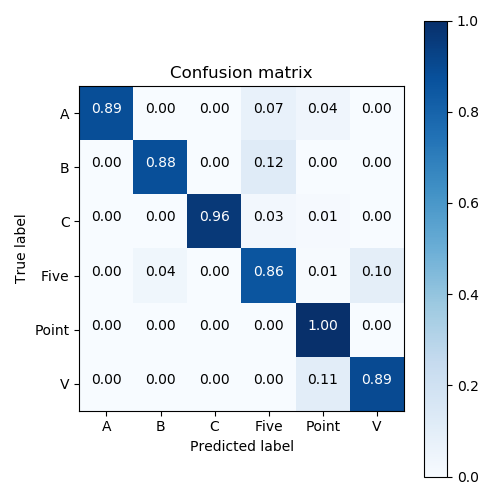
\includegraphics[width=5cm]{figs/confusion_matrix_xception2.png} 
\end{tabular}
\end{center}
\caption{Matriz de confusão para o modelo Xception que obteve a maior acurácia.}
\label{fig:res1}
\end{figure}

\subsection{Reconhecimento Baseado em Parâmetros de Forma}
O método foi avaliado utilizando as imagens do conjunto de teste para comparação com o desempenho do método de utilizando redes neurais convolucionais. A Tabela \ref{tab:res2} resume os resultados obtidos utilizando o método descrito em ~\cite{shapeparameters}.

\begin{table}[htbp]
\centering
\caption{Resultados obtidos usando Shape Parameters.}
\label{tab:res2}
\begin{tabular}{|c|c|}
\hline
Gesto & Acurácia    \\\hline
A       & 16.7\%   \\\hline
B       & 0.0\%    \\\hline
C       & 0.0\%    \\\hline
Five    & 10.4\%   \\\hline
Point   & 37.0\%   \\\hline
V       & 38.9\%   \\\hline
\textbf{Total} & \textbf{16.9\%} \\\hline
\end{tabular}
\end{table}

\begin{figure}[htbp]

\begin{tabular}{c}
	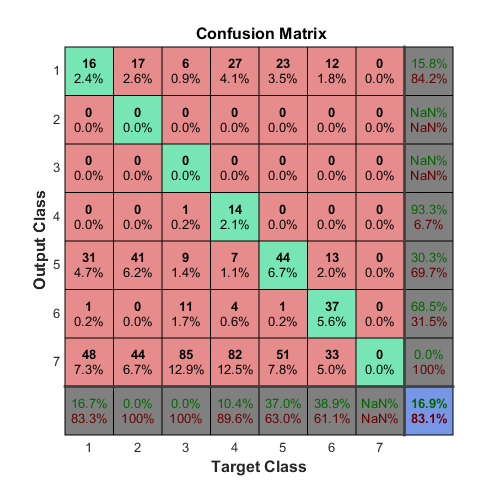
\includegraphics[width=8cm]{figs/confusion_matrix.png} 
\end{tabular}
\caption{Matriz de confusão para o método utilizando \textit{shape parameters}. As classes enumeradas de 1 a 6 são [A, B, C, FIVE, POINT, V], respectivamente, enquanto a classe 7 representa falhas de segmentação/classificação.}
\label{fig:res2}
\end{figure}

\par Como mostrado na tabela, observa-se que as taxas de acerto para todos os gestos foram insatisfatórias, tendo gestos que não foram reconhecidos em nenhuma tentativa.   

\section{Conclusão}
% Resumir projeto e discussões
Os resultados obtidos para o modelo utilizando Redes Neurais Convolucionais foram satisfatórios, visto que a melhor acurácia relatada por \cite{hand} foi de 78.22\%. Enquanto que para o modelo que utiliza parâmetros de forma, a acurácia alcançada foi muito baixa. O fato do modelo ter sido desenvolvido para reconhecimento de gestos em fundo uniforme e com a mão reta e de frente para a câmera influenciou diretamente na segmentação da mão. Pois no dataset testado, poucas imagens apresentavam uniformidade no fundo juntamente com a correta posição da mão em relação a câmera. Dessa forma, a segmentação foi prejudicada, o que ocasionou em resultados baixos de acerto no reconhecimento dos gestos. Uma outra forma de segmentação, adequada a fundos heterogêneos, é o indicado para aumentar as taxas de acerto deste modelo.  
\par Dessa forma, é correto concluir que o método utilizando Redes Neurais Convolucionais é mais adequado para ser utilizado em reconhecimento de gestos quando o ambiente das imagens não é um ambiente controlado.

\bibliography{refs}{}
\bibliographystyle{plain}
\end{document}
